\chapter{Конструкторская часть}

\section{Разработка алгоритма сортировки слиянием}

На рисунке \ref{img:merge} приведена схема алгоритма сортировки слиянием.
\begin{figure}[h]
	\centering
	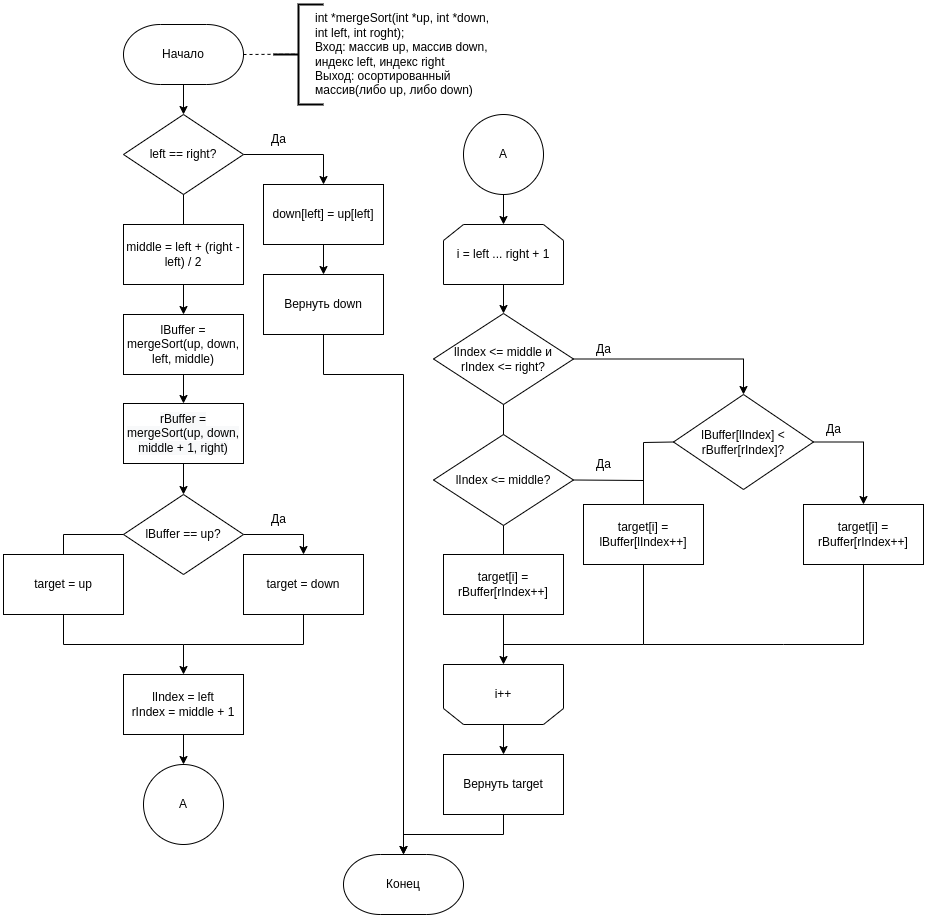
\includegraphics[width=170mm]{images/merge}
	\caption{Схема алгоритма сортировки слиянием.}
	\label{img:merge}
\end{figure}
\newpage
На рисунке \ref{img:counting} приведена схема алгоритма сортировки подсчетом.
\begin{figure}[h]
	\centering
	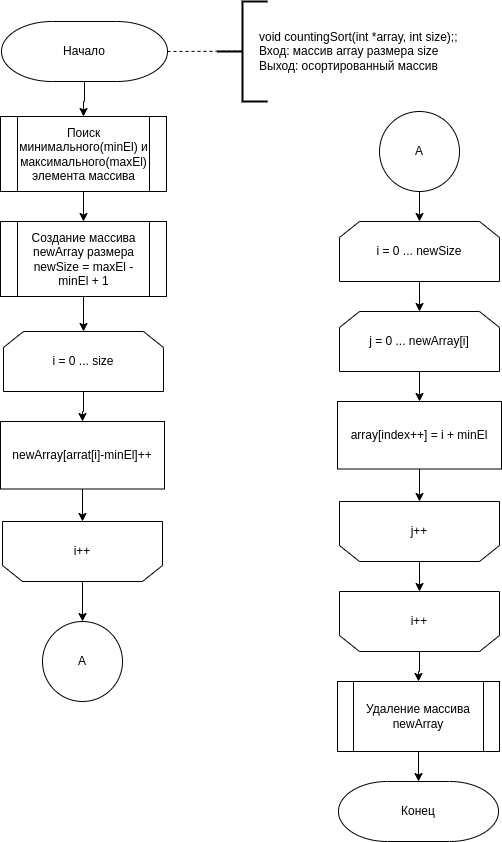
\includegraphics[width=110mm]{images/counting}
	\caption{Схема алгоритма сортировки подсчетом.}
	\label{img:counting}
\end{figure}

\newpage
На рисунке \ref{img:bitonic} приведена схема алгоритма битонной сортировки.
\begin{figure}[h]
	\centering
	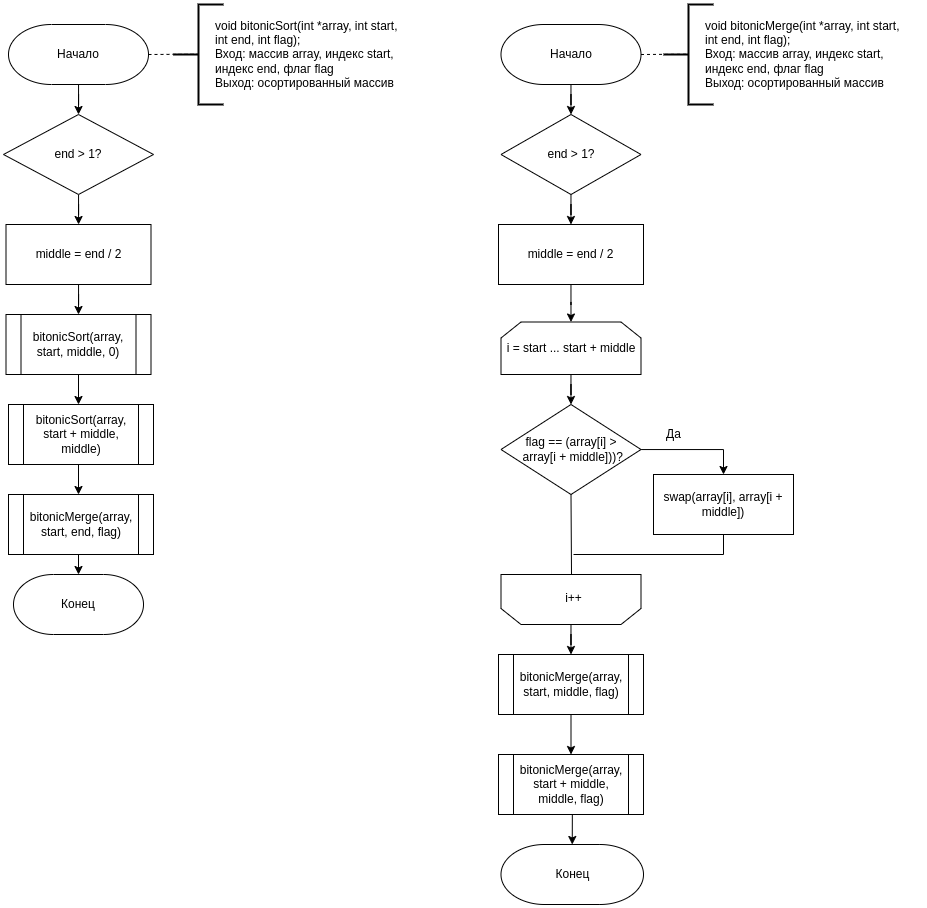
\includegraphics[width=175mm]{images/bitonic}
	\caption{Схема алгоритма битонной сортировки.}
	\label{img:bitonic}
\end{figure}

\section{Модель вычислений}

Для последующего вычисления трудоемкости необходимо ввести модель вычислений.

Операции из списка (\ref{for:opers}) имеют трудоемкость 1:
\begin{equation}
	\label{for:opers}
	=, +=, -=, +, -, *, /, \%, ==, !=, <, >, <=, >=, [], ++, {-}-
\end{equation}

Трудоемкость оператора выбора \code{if условие then A else B} рассчитывается как:
\begin{equation}
	\label{for:if}
	f_{if} = f_{\text{условия}} +
	\begin{cases}
		f_A, & \text{если условие выполняется,}\\
		f_B, & \text{иначе.}
	\end{cases}
\end{equation}

Трудоемкость цикла рассчитывается как:
\begin{equation}
	\label{for:for}
	f_{for} = f_{\text{инициализации}} + f_{\text{сравнения}} + N \cdot (f_{\text{тела}} + f_{\text{инкремента}} + f_{\text{сравнения}})
\end{equation}

Трудоемкость вызова функции равна 0.

\section{Трудоемкость алгоритмов}

Далее размер массива обозначается как $size$.

\subsection{Алгоритм сортировки слиянием}

\subsection{Алгоритм сортировки подсчетом}

Трудоемкость алгоритма сортировки подсчетом состоит из:

\begin{itemize}
	\item трудоемкость поиска минимального элемента в массиве:
	\begin{equation}
		\label{min}
		f_{min} =  2 + size \cdot (f_{\text{тела}} + 2)
	\end{equation}

	\item трудоемкость поиска максимального элемента в массиве:
	\begin{equation}
		\label{max}
		f_{max} =  2 + size \cdot (f_{\text{тела}} + 2)
	\end{equation}
			
	\item трудоёмкость каждой итерации цикла поиска минимального и максимального элемента:
	\begin{equation}
	\label{min_max_if}
	f_{\text{тела}} = 4 + \begin{cases}
		0, & \text{в лучшем случае},\\
		2, & \text{в худшем случае}.\\
	\end{cases}
	\end{equation}

	\item трудоемкость заполнения временного массива:
	\begin{equation}
		\label{newArray}
		f_{\text{доп}} = 2 + size \cdot (4 + 2) = 2 + 6 \cdot size
	\end{equation}

	\item трудоемкость внешнего цикла заполнения массива:
	\begin{equation}
		\label{array}
		f_{\text{массив}} = 2 + newSize \cdot (f_{\text{внутренний}} + 2) 
	\end{equation}

	\item трудоемкость внутреннего цикла заполнения массива:
	\begin{equation}
		\label{innerArray}
		f_{\text{внутренний}} = 3 + size \cdot (3 + 4)  = 3 + 7 \cdot size 
	\end{equation}
	
	\item суммарная трудоёмкость внешнего и внутреннего циклов:
	\begin{equation}
		\label{array}
		f_{\text{суммарная}} = 2 + newSize \cdot (5 + 7 \cdot size) 
	\end{equation}
\end{itemize}

Трудоёмкость в лучшем (массив отсортирован, все элементы совпадают) случае:

\subsection{Алгоритм битонной сортировки}